%\documentclass[]{IEEEphot}
\documentclass[conference]{IEEEtran}
\usepackage[utf8]{inputenc}
\usepackage[parfill]{parskip}
\usepackage{tikz}
\usepackage{amssymb}

%\jvol{xx}
%\jnum{xx}
%\jmonth{November}
%\pubyear{2011}

\begin{document}
\title{Clustering Algorithms Overview}
\author{Mentor, Primož, Matej}
%\affil{Fakulteta za računalništvo in informatiko}  
\maketitle

\begin{abstract}
Abstract is missing!
\end{abstract}

\begin{IEEEkeywords}
Machine learning, clustering, k-means, ECMC, Expectation Maximization.
\end{IEEEkeywords}

\section{Introduction}
What is clustering? It's an unsupervised machine learning task. Computationally difficult
(NP-hard). Heuristic algorithms. Iterative refinements. Clustering algorithms taxonomy.

Clustering refers to the problem of partitioning a dataset into subsets, such that members
within subsets are more similar to each other (according to some criterion) than to members
of other subsets. Each subset is called a cluster.

Clustering is recognized as an important tool in areas such as image segmentation,
speech recognition, signal compression, medical research, document storage and retrieval,
world-wide-web search and mining and bioinformatics.

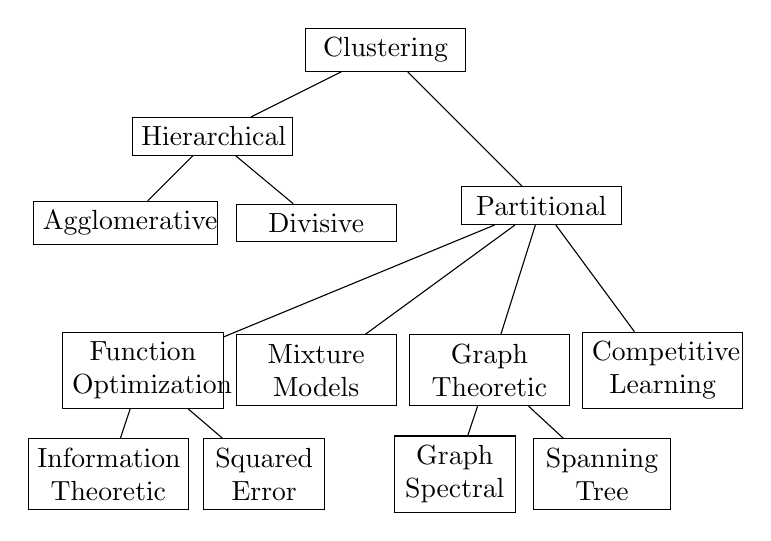
\begin{tikzpicture}[scale=1.1, text width=1.8cm, text centered]
    \tikzstyle{every node} = [rectangle,draw]

    \node (a) at (7, 5) {Clustering};
    \node (b) at (5, 4) {Hierarchical};
    \node (c) at (8.8, 3.2) {Partitional};

    \node (d) at (4, 3) [text width=2.1cm] {Agglomerative};
    \node (e) at (6.2, 3) {Divisive};

    \node (f) at (4.2, 1.3) {Function \\ Optimization};
    \node (g) at (6.2, 1.3) {Mixture \\ Models};
    \node (h) at (8.2, 1.3) {Graph \\ Theoretic};
    \node (i) at (10.2, 1.3) {Competitive \\ Learning};

    \node (j) at (3.8, 0.1) {Information \\ Theoretic};
    \node (k) at (5.6, 0.1) [text width=1.3cm] {Squared \\ Error};

    \node (l) at (7.8, 0.1) [text width=1.3cm] {Graph \\ Spectral};
    \node (m) at (9.5, 0.1) [text width=1.5cm] {Spanning \\ Tree};

    \draw [-] (a) -- (b);
    \draw [-] (a) -- (c);

    \draw [-] (b) -- (d);
    \draw [-] (b) -- (e);

    \draw [-] (c) -- (f);
    \draw [-] (c) -- (g);
    \draw [-] (c) -- (h);
    \draw [-] (c) -- (i);

    \draw [-] (f) -- (j);
    \draw [-] (f) -- (k);

    \draw [-] (h) -- (l);
    \draw [-] (h) -- (m);
\end{tikzpicture}

\section{Clustering performance evaluation}
TODO: external/internal evaluation

\subsection{Adjusted Rand Index}
Rand Index (RI) is a measure of similarity between data clusterings. It counts
the number of agreements between two clusterings:

$RI = \frac{a+b}{{n \choose 2}}$

where
\begin{itemize}
    \item \textit{a} is the number of pairs of elements (points, examples) that are in the same cluster in the first clustering
    as well as in the other clustering,
    \item \textit{b} is the number of pairs of elements that are in different clusters in both clusterings,
    \item \textit{n} is the number of elements.
\end{itemize}

Adjusted Rand Index (ARI) is the corrected-for-chance version of RI.
ARI has the advantage over plain RI in that it scores random 
clusterings close to 0 for any number of clusters and data samples. It returns
a value in range $[-1, 1]$, where negative values are bad, similar clusterings have
positive values and 1.0 is the perfect match score. ARI makes no assumption on the cluster
structure and can therefore be used to compare different algorithms such as K-means (which
constructs isotropic clusters) with spectral or other algorithms (which can find non-convex
clusters).

\subsection{Homogeneity, completeness and V-measure}
Rosenberg and Hirschberg (2007) defined two desirable objectives of clustering: homogeneity and
completeness. Homogeneity refers to a desire that each cluster should contain only members
of a single class whereas completeness expresses the aspiration that all members of a given
class are assigned to the same cluster.
%\begin{itemize}
%    \item \textbf{homogeneity}: each cluster contains only members of a single class and
%    \item \textbf{completeness}: all members of a given class are assigned to the same cluster.
%\end{itemize}
We can translate these objectives to math in the following way:

$homogeneity = 1 - \frac{H(C|K)}{H(C)}$

$completeness = 1 - \frac{H(K|C)}{H(K)}$

where $H(C|K)$ is the conditional entropy of the classes given the cluster assignments defined as:

$H(C|K) = - \sum\limits_{c=1}^{|C|}\sum\limits_{k=1}^{|K|}\frac{n_{c,k}}{n}\cdot \log{\frac{n_{c,k}}{n_k}}$

and $H(C)$ is the entropy of the classes:

$H(C) = - \sum\limits_{c=1}^{|C|}\frac{n_c}{n} \cdot \log{\frac{n_c}{n}}$

with $n$ the total number of examples, $n_c$ and $n_k$ the number of examples belonging to class
$c$ and cluster $k$ respectively, and with $n_{c,k}$ the number of examples from class $c$ assigned
to cluster $k$.

The conditional entropy of clusters given class $H(K|C)$ and the entropy of clusters $H(K)$ are
defined in a symmetric manner.

Rosenberg and Hirschberg (2007) defined V-measure as the harmonic mean of homogeneity and completeness:

$v = \frac{2 \cdot h \cdot c}{h+c}$

Advantages of these measures are bounded scores ($[0, 1]$, 1.0 means perfect score), intuitive interpretation and that
no assumption is made on cluster structure (similar to ARI). Unfortunately, they are not normalized
with respect to random clustering: random clustering will not yield the same values and it won't
yield zero score when the number of clusters is large compared to the number of samples. For smaller
sample sizes or larger number of clusters it is better to use an adjusted measure such as ARI.

\section{Algorithms}
\subsection{K-means}
K-means clustering (KMC) is a simple and well known algorithm. It is usually very
fast (commonly run multiple times with different starting conditions), but tends
to produce spherical clusters with similar size, which can be undesirable.
k-means is often used as a preprocessing step for other algorithms. The standard
algorithm was first proposed by Stuart Lloyd in 1957 and published later in 1982.

%The number of clusters we want to find in data is fixed a priori ($k$).
KMC requires as input the number of cluster we want to find in data ($k$).
The algorithm iteratively refines clusters' locations (guided by a cost function),
until no more refinements are possible (clusters do not change anymore)
or max number of iterations has been reached. It can be summarized as [Jain et al., 2000]:

\begin{enumerate}
    \item Select an initial partition with k clusters.
    \item Generate a new partition by assigning each example to its closest cluster center.
    \item Compute new cluster centers as the centroids of the clusters.
    \item Repeat step 2 and 3 until convergence.
\end{enumerate}
%$m_1^{(1)}$, $m_2^{(1)}$, ..., $m_k^{(1)}$
%denote centroids (also called means). The superscript index denotes the current iteration.
%$S_i^{(t)}$ is a cluster (set of examples) with the corresponding centroid $m_i^{(t)}$.
%There are two alternating steps in the algorithm:

%\begin{itemize}
%\item \textbf{Assignment step}\\
  %Each example is assigned to the cluster with the closest centroid:\\
  %$S_i^{(t)} = \{x_j : ||x_j - m_i^{(t)}|| \le ||x_j - m_l^{(t)}|| \forall l = 1, ..., k\}$
%\\
%\item \textbf{Update step}\\
  %New means are calculated and set as centroids:\\
  %$m_i^{(t+1)} = \frac{1}{|S_i^{(t)}|} \displaystyle\sum\limits_{x_j \in S_i^{(t)}}{x_j}$
%\end{itemize}

There are two common ways to select the initial centroids: random seed and random partition.
The random seed method randomly chooses k observations from the data set
and uses these as the initial means. Random partition
assigns each example into one of the k clusters randomly.
The random seed method tends to spread the initial means out, while random partition
places all of them close to the center of the data set.

There are also better approaches to initialization: k-means++ algorithm specifies a
procedure to initialize the cluster centers before proceeding with the standard k-means
optimization iterations. With the k-means++ initialization, the algorithm is guaranteed
to find a solution that is $O(\log k)$ competitive to the optimal k-means solution.
Although this initial selection takes extra time, it speeds up the convergence and 
therefore actually lowers overall computation time.

Although it can be proved that the KMC algorithm will always terminate (converge),
it does not necessarily find the most optimal configuration,
corresponding to the global objective function minimum. The algorithm is also sensitive
to the initial selected cluster centroids but it can be run multiple times to reduce this effect.

Another interesting fact is that, in the worst case, k-means can be very slow to converge:
in particular it has been shown that there exist certain datasets,
even in 2 dimensions, on which k-means takes exponential time to converge.
These datasets do not seem to arise in practice: this is supported by the
fact that the smoothed time complexity of k-means is polynomial.

\subsection{Evolving Clustering Method}

ECM (Evolving Clustering Method) is dynamic clustering method mostly used for on-line system with fast "one-pass" algorithm. It's extension ECMc (Evolving Clustering Method with Constrained minimization) is used for off-line where constrained optimisation is applied. Both ECM and it's extension were introduced in 2001 by Qun Song and Nikola Kasabov.

ECM is a distance based clustering method where each cluster has a centre, where all of cluster's members are less distant from the centre than $D_{thr}$. $D_{thr}$ is by default input in algorithm, unlike to some others where number of cluster is input. However, $D_{thr}$ does affect number of clusters but not directly. Therefore, when comparing ECM algorithm to others you have to be aware of their inputs.

ECM takes samples from a data stream and with every new data cluster's radius can be updated or it's center changed or new cluster can be created. At some point, usually when cluster radius reaches threshold value $D_{thr}$, cluster radius will not update anymore.

Both ECM and ECMc consist of several steps where ECM is a pre-process to ECMc. First sample is used to create first cluster with radius 0 and centre on the sample itself. For every new sample $x_i$ next steps are taken:
\begin{enumerate}
\item Distance from $x_i$ to every cluster centre is calculated as shown in equation \ref{ECMdist}.
\item If minimum distance found is less than or equal to cluster radius, $x_i$ belongs to cluster and algorithm returns to step 1.
\item For every cluster s is calculated as shown in equation \ref{ECMequ1}. If minimum s is more than $2*D_{thr}$ a new cluster is created and algorithm continues at step 1.
\item Cluster's centre, with minumum s calculated, is moved and radius increased. New radius is calculated as $s/2$ and centre's position is on the line from old centre to sample $x_i$ so that distance from new centre to point $x_i$ is equal to $s/2$ as shown in equation \ref{ECMequ2} and \ref{ECMequ3}.
\end{enumerate}

\begin{equation}\label{ECMdist}
dist(i,j) = \sqrt{ \frac {\sum_{d=1}^{D} (x_i^d - C_{cj}^d)^2} {D}}
\end{equation}

\begin{equation}\label{ECMequ1}
s(i, j) = dist(i,j) + radius(C_j)
\end{equation}

\begin{equation}\label{ECMequ2}
f = 1 - \frac {\frac {s} {2}} {\sqrt{ \sum_{d=1}^{D} (C_c^d - x_i^d)}}
\end{equation}
\begin{equation}\label{ECMequ3}
Cc^d = Cc^d + (f * (x_i^d - C_c^d))
\end{equation}

This way it holds for each sample in its own cluster that the distance between centre and sample is less than or equal to $D_{thr}$. Afterwards constrained optimisation can be applied to minimize the function \ref{ECMJ}. For optimisation the following steps have to be taken:
\begin{enumerate}
\item 1. Change the membership of each sample in data to cluster that has the smallest distance to it's centre
\item 2. Calculate new cluster centre to fit new changes
\item 3. The end of algorithm is reached if enough iterations occured or the change of function \ref{ECMJ} is less than certain amount. Otherwise continue with going back to step 1.
\end{enumerate}

\begin{equation}\label{ECMJ}
J = \sum_{k=1}^K \sum_{i=1}^{N_{Ck}} dist(x_{ki}, C_{ck})
\end{equation}

\subsection{Expectation Maximization Gaussian Mixture Model}

\subsection{Spectral Clustering}
Spectral clustering has become more popular in recent years. It uses standard linear algebra
methods, it is relatively simple to implement and its results are often better than those of
traditional clustering approaches (such as K-means). In short, spectral clustering exploits the
eigenvalues and eigenvectors (called spectrum of a matrix, hence the name) of the similarity matrix
(which represents
a measure of similarity between examples) of the data to perform dimensionality reduction for
clustering in low-dimensional space. It is not obvious to see why it works at all
and we will not dive into details in this article, instead we will try to give a high level overview.
An intuitive explanation from three different theoretic backgrounds is given by [Luxburg, 2007].

Similarity graphs and graph Laplacians are the key tools in spectral clustering.
Similarity graph is constructed from data by interpreting examples as vertices and similarities
between examples as weighted edges between vertices. This enables reformulating the problem
of clustering: we want to find a partition of the graph such that the edges between different groups
have low weights (dissimilar examples) and the edges within a group have high weights (similar examples).
There are several ways of building these graphs:
\begin{itemize}
    \item $\epsilon$-neighborhood graph: All examples whose pairwise distances are smaller than $\epsilon$
    are connected. In practice it can be difficult to choose a useful value for $\epsilon$. Setting it too
    low might fail to connect sparse clusters, whereas setting it too high might unnecessarily connect many
    examples (different scales problem).
    \item $k$-nearest neighbor graph: Each example is connected with its nearest $k$ examples. Recommended
    by [Luxburg, 2007].
    \item Fully connected graph: Simply connecting all examples with each other. Results in a dense matrix.
\end{itemize}

% TODO: connection with graph cut!

Graph Laplacian matrices are studied in Spectral graph theory. They encode graph adjacency information
as well as information about degrees of vertices and have some interesting properties used in spectral
clustering, e.g. the multiplicity of the eigenvalue 0 equals the number of connected components in the graph
[Mohar, 1991, 1997].

There are several variants of spectral clustering algorithms. We will describe only unnormalized version
as presented in [Luxburg, 2007]. Given similarity matrix $S \in \mathbb{R}^{n \times n}$ and the number
of clusters to construct $k$:

% TODO: refer to authors of different variants

\begin{itemize}
    \item Construct a similarity graph.
    \item Compute the unnormalized Laplacian L.
    \item Compute the first $k$ eigenvectors $u_1, \dots, u_k$ of $L$ and combine them into
    $U \in \mathbb{R}^{n \times k}$ as columns.
    \item Cluster rows of $U$ ($y_i \in \mathbb{R}^k$ is the $i$-th row) with the K-means algorithm
    into clusters $C_1, \dots, C_k$.
    \item Output are clusters $A_1, \dots, A_k$, where $A_i = \{ j|y_j \in C_i \}$
\end{itemize}

The main trick of this algorithm is to change the representation of the examples to $y_i \in \mathbb{R}^k$.
In this new representation clusters can be easily detected, even by a simple algorithm such as K-means.

Spectral clustering is being given a lot of attention mainly because it does not make strong
assumptions on the form of the clusters. Unlike many other clustering algorithms it
can solve very general problems like intertwined spirals.
Spectral clustering can be implemented efficiently even for large datasets, as long as
the similarity graph is sparse. Once the similarity graph is chosen, a linear problem needs to
be solved. There are no issues of getting stuck in a local minima and there is no need to
restart the algorithm several times with different initializations. However, choosing
a good similarity graph is not trivial, and spectral clustering can
be quite unstable under different choices of the parameters for the neighborhood graphs.

\subsection{Information Theoretic Clustering}%Cauchy-Schwarz Divergence Clustering}
KMC and similar are examples of so-called \textit{parametric} methods of clustering. These
methods assume some knowledge about clusters' structure, which makes them less
suitable for many use cases. KMC performs badly when clusters are not hyperelliptical
because it implicitly assumes Gaussian cluster distributions. In fact, any clustering method
that utilizes second order data statistics can produce only convex clusters [Jain et al., 2000].

Information theory has been successfully used in clustering by several researchers in recent years.
Various information-theoretic clustering metrics, such as entropy, mutual information and
Kullback-Leibler divergence were researched.

[Faivishevsky \& Goldberg, 2010] suggested an algorithm based on maximizing the mutual information
between examples and clusters. Their method does not impose any parametric model on the cluster
distribution because they used a non-parametric estimation of the average cluster entropies (MeanNN,
by the same researchers, 2009). Their algorithm starts with random partitioning and continues
with reassigning examples between clusters, trying to improve the cost function they developed,
until improvements become sufficiently small. Algorithm's overall computational complexity is
$O(n^2)$, but it is able to cluster non-convex data sets.

Another group of algorithms was developed by [Jenssen et. al, 2005, 2010]. They combined
the Renyi entropy [Renyi, 1976], which is an information theoretic measure of uncertainty of a random variable,
and the well known Cauchy-Schwarz inequality, forming Cauchy-Schwarz pdf (probability density function)
divergence measure (statistical distance). The measure between two cluster pdf's $p(x)$ and $q(x)$ is defined as:

$D_{CS}(p, q) = -\log \frac{\int p(x)q(x)dx}{\sqrt{\int p^2(x)dx \int q^2(x)dx}}$

This divergence can be regarded as an approximation of Kullback-Leibler divergence between two pdf's [Jenssen, 2009].
An intuitive reasoning behind this measure is that in order to optimize $D_{CS}$, the entropy of each individual cluster must
be small, while at the same time the entropy across the clusters must be large.
Probability densition functions can be estimated by a sample-based estimator. [Jenssen, 2010] used a kernel
density estimator developed by [Parzen, 1962] (Parzen-Rosenblatt window technique). This introduces a problem of
choosing the kernel size (this is a problem of all kernel-based methods).

An early idea to maximize the Cauchy-Schwarz pdf divergence was to seed a number
of small initial clusters in the data set, grow clusters (assigning examples to clusters
in a way that maximizes the divergence) until all examples have been clustered, and then
reassign the members of the worst cluster (decided again by the divergence), reducing the number of clusters. 
The reassigning step is repeated until the desired number of clusters is reached.

[Jenssen et at., 2007] derived an optimization procedure based on the technique of Lagrange multipliers.
This resulted in an efficient gradient descent-based clustering algorithm which incorporated kernel annealing
as an optimization strategy. The kernel size may start large during the initial iterations, but then annealed (reduced)
in following iterations. The annealing procedure can also help the algorithm to cope with different data scales,
by discovering large scale structures first, followed by fine tuning as the kernel size is decreased.

The main advantage of these clustering approaches is that the underlying clustering metric is
based on entropy. Entropy conveys information about the shape of probability distribution,
and not only variance (which e.g. K-means rely on). This enables the clustering of data sets consisting of
elongated and highly irregular clusters.

% TODO: connection with graph-theoretic approaches

\section{Results}

\section{Conclusions}

\section*{Acknowledgements}
Thanks to TODO.

\section*{References}

\end{document}
